\chapter{Modular System Structure}
\label{chap:modular-structure}
% Traceability: ADR-001 ADR-002 ADR-003 ADR-004 ADR-005 ADR-006

The controller is divided into parts that can be designed, tested, and replaced separately. This is the main purpose of the modular structure. It allows the system to change over time without turning every upgrade into a complete controller redesign.

Modularity depends on clear boundaries. A removable board is not truly independent if changing it also requires undocumented changes in several other boards. The architecture therefore assigns each system responsibility to an owner and places shared behavior in controlled interfaces.

Figure~\ref{fig:modular-cards} gives a simple physical picture of the modular idea. A main board and specialized function boards plug into a common backplane. The drawing is conceptual: the number, size, and arrangement of boards depend on the instrument.

\begin{figure}[htbp]
  \centering
  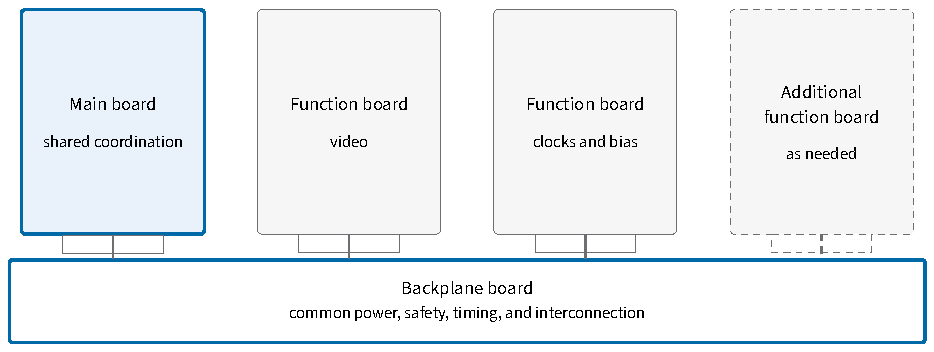
\includegraphics[width=0.92\textwidth]{figures/generated/modular_cards.tikz.pdf}
  \caption{Conceptual modular arrangement. The backplane provides the common platform, while removable boards provide coordination or detector-specific functions.}
  \label{fig:modular-cards}
\end{figure}

Figure~\ref{fig:system-overview} shows how these physical elements connect to the wider instrument. This chapter explains the responsibilities behind the structure.

\section{A Stable Platform with Specialized Function Boards}

The architecture separates common platform services from detector-specific electronics.

The common platform provides protected power, utility rails, safety coordination, timing distribution, communication access, and mechanical connections. These services are useful to many detector systems and should behave consistently.

Function boards provide the electronics that depend on the detector. A system may use video boards, clock boards, bias boards, or a board that combines several functions. A new detector may require a new function board without requiring a new main board or a new backplane architecture.

This separation does not mean that every function board is simple or identical. It means that each board connects to the rest of the controller through a known set of contracts. A board uses only the shared resources it needs and provides the safety, timing, communication, and electrical behavior required for its role.

\section{Main Board}

The main board coordinates system-wide actions. It generates or distributes the signals that must be common across several function boards.

Its main responsibilities are:

\begin{itemize}
  \item driving the shared arm and recovery signals;
  \item generating the acquisition clock and synchronization events;
  \item providing synchronization signals for the backplane utility converters;
  \item monitoring the shared fault bus and continuity loop;
  \item measuring common power rails for diagnosis; and
  \item communicating with the host as its own active board.
\end{itemize}

Detector sequencers, detector-specific electronics, video processing, and science-data transport belong to function boards. Main coordinates shared actions.

This limited role is important for scaling. Replacing a video board with a faster design should not require a faster main-board data path. Adding a detector-specific function should not require adding that function to the main board.

The main board can coordinate shared electrical behavior without knowing which logical instrument role is installed in each slot. The host owns that inventory. This keeps physical position separate from operational identity.

\section{Function Boards}

A function board performs work that is specific to a detector or instrument. Typical examples include:

\begin{itemize}
  \item digitizing detector video;
  \item generating detector clocks;
  \item generating detector bias voltages;
  \item controlling detector support electronics; or
  \item combining several related functions when an instrument needs it.
\end{itemize}

Each active function board contains the processing, firmware, local conversion, monitoring, and network connection needed for its own work. It receives common timing and coordination signals from the platform, but it decides locally whether it is ready to operate. It also participates directly in the shared hardware safety path.

A function board does not command another function board. Coordination comes from the host and the shared signals driven by the main board. This avoids hidden dependencies between particular board types.

Function boards are also responsible for their detector interfaces. Their ICDs define voltage ranges, timing, loading, data capacity, and other limits at those interfaces. Specialized detector voltages remain local to the board that needs them. Common rails are used only when they fit the function and noise requirements.

The host configures each function board and reads its diagnostics directly. Chapter~\ref{chap:identity-data} explains communication and science-data transport.

\section{Example: Inside a Function Board}

A function board is a removable PCB assembly connecting the common controller infrastructure to a detector function. Figure~\ref{fig:example-function-board} uses a video board to show what that means. The outline and zones explain the parts and their relationships; they are not a PCB placement plan.

The backplane connector carries fixed power contacts, timing and coordination signals, \texttt{OK}, returns, and continuity-loop contacts. Local conversion supplies ordinary digital loads from protected \texttt{+12V}. Analog loads may use the shared utility rails, local conversion, or both.

Processing and memory configure the function, capture or process samples, and handle host traffic. Timing hardware receives acquisition events, while local management and safety clocking remains independent where required. Interlock hardware includes the watchdog, fail-safe paths, supply supervision, and an optional dedicated safety CPLD. It controls applicable detector-facing permissives independently of ordinary processing.

The functional electronics in this example comprise input protection, analog conditioning, an ADC, and local monitoring. The detector interface connector links them to the detector or preamplifier. Ethernet connects directly to the host; UART provides local commissioning and recovery. The continuity path may use passive copper or unconditional hardware forwarding in the safety CPLD. It is independent of software and operating state.

\begin{figure}[htbp]
  \centering
  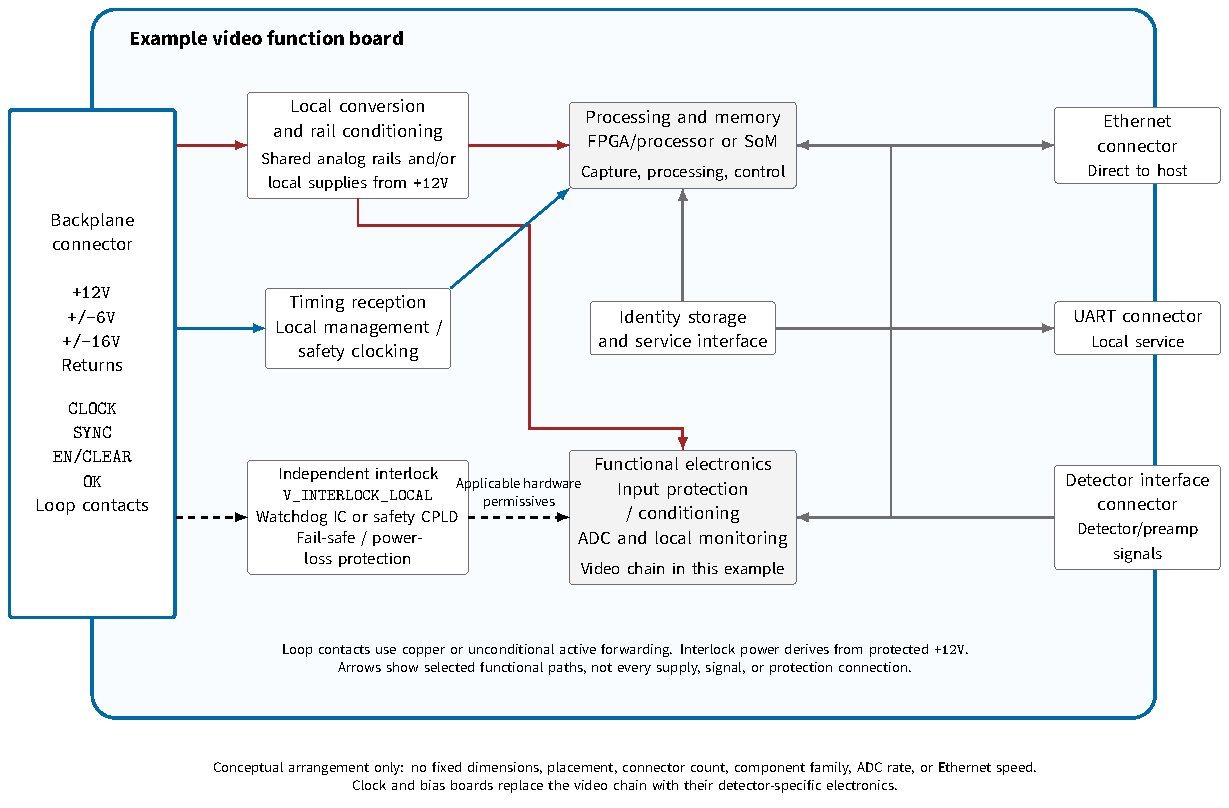
\includegraphics[width=\textwidth]{figures/generated/example_function_board.tikz.pdf}
  \caption{Conceptual video function board with its connectors and main functional parts. Arrows show selected relationships, not complete wiring. Dimensions, component choices, connector geometry, sampling rate, and link speed remain application-specific.}
  \label{fig:example-function-board}
\end{figure}

A clock or bias board replaces the video chain with drivers or DAC/output stages. The common interfaces retain the same meaning. A local voltage/current monitor does not replace analog input protection, and the illustration does not prescribe a relay circuit or processor family.

\section{Backplane Board}

The backplane is more than a passive collection of connectors. It provides the common physical and power infrastructure for the controller.

Its responsibilities include:

\begin{itemize}
  \item protecting the external power input and distributing protected bulk power;
  \item generating the standard utility rails;
  \item supervising the shared rails and contributing faults directly to the shared safety bus;
  \item routing timing, coordination, safety, and continuity signals;
  \item providing the electrical and mechanical slot interface; and
  \item maintaining deliberate analog, digital, return, and shielding paths.
\end{itemize}

The utility converters live on the backplane because their rails are common platform resources. Boards that need high-current digital power create it locally from protected bulk power. This avoids sending large processor and FPGA currents through low-voltage shared-rail contacts.

The backplane does not interpret instrument commands or control detector operation. Its active circuits provide power, protection, supervision, and signal distribution. Detailed thresholds, connector assignments, current limits, and routing rules belong to the backplane ICD and hardware design.

Every standard backplane presents the same set of common rails, even when a particular function board does not use all of them. Removing or changing a standard rail creates an architecture variant rather than a normal board option. This single definition keeps board and backplane documentation manageable.

\section{Bridge Boards and Additional Backplanes}

A bridge board allows the controller to use another backplane when one backplane is not enough. It carries the supported shared interfaces across the extension and reproduces active signals where required.

The extension must preserve the meaning of the original interfaces. The shared fault bus remains one hardware interlock. The continuity loop must travel through the extension and return to the main board, so a disconnected cable is detected. Timing must still reach each supported slot through a verified point-to-point path.

A bridge board is an active board and therefore has its own communication, health monitoring, watchdog, and local interlock power. Its continuity path may use passive copper or qualified active forwarding. A bridge power failure trips through a separate local hardware contribution or through active forwarding and main-board conversion, respectively.

The architecture does not set one universal number of slots or backplanes. Each instrument selects a topology and verifies the complete power, timing, network, thermal, and mechanical budgets. An available connector does not prove that the system has capacity for another board.

\section{Passive Terminators and Unused Slots}

The continuity loop passes through every slot. An unused slot therefore needs a passive terminator to complete the loop. The terminator is a small unpowered insert with the required copper connection. It is not an active board and has no identity, network connection, or local interlock supply.

Removing a board or terminator breaks the loop and places the system in a safe condition. Live insertion and removal are not normal operating modes. Board replacement is performed with the controller powered down or already safely latched.

\section{Responsibility Boundaries}

Table~\ref{tab:responsibility-boundaries} summarizes the main ownership rules. The goal is not to list every circuit. It is to show where a design change should begin and which interface must remain stable.

\begin{table}[htbp]
\centering
\small
\begin{tabularx}{\textwidth}{@{}>{\bfseries\raggedright\arraybackslash}p{0.19\textwidth}>{\raggedright\arraybackslash}p{0.31\textwidth}>{\raggedright\arraybackslash}X@{}}
\toprule
Owner & Owns & Does not own \\
\midrule
Remote host & Instrument inventory, configuration, operation, and data reception & Hardware interlock action or board-local safety decisions \\
Main board & Shared enable, recovery, acquisition timing, synchronization, and continuity-loop monitoring & Detector sequencers, detector-specific electronics, or science-data concentration \\
Function board & Its detector function, local readiness, local protection, diagnostics, and direct host traffic & System-wide signal generation or control of other function boards \\
Backplane board & Protected power, common utility rails, shared-rail supervision, slots, and common routing & Instrument commands or detector-specific behavior \\
Bridge board & Verified extension of supported interfaces to another backplane & Redefinition of those interfaces or independent system coordination \\
Passive terminator & Continuity through an unused slot & Any powered or programmable function \\
\bottomrule
\end{tabularx}
\caption{High-level ownership boundaries. Exact interfaces and limits are defined in the applicable ICDs.}
\label{tab:responsibility-boundaries}
\end{table}

These boundaries make common changes easier to contain:

\begin{itemize}
  \item An obsolete processor can be replaced inside a board design if the board still meets its interfaces.
  \item A new detector can use a new function board while reusing the common platform.
  \item More channels can be added by composition after the complete system budgets are checked.
  \item A change to a shared signal, rail, or board role is an architecture or ICD change because it affects several independent elements.
\end{itemize}

System integration verifies that the installed boards meet their declared interface and capacity limits.

\medskip
\noindent\textit{Chapter sources:} ADR-001 through ADR-006, with the main ownership rules in ADR-002 through ADR-005. The repository README defines the document and terminology boundaries.
